\section{\large Unidad I. Categorización de los Fundamentos de la Geometría}

En la Geometría Moderna se asumen como términos primitivos o indefinidos, es decir como punto de partida, los conceptos de \textbf{Punto, Recta} y \textbf{Plano}.

Cada uno de estos términos son una idea, una noción o una abstración de lo que son.
Nunca nadie ha ``visto'' un punto, una recta o un plano en su vida, porque estos solo existe en la mente.

Un \textbf{punto} decimos que es una posición en el espacio, sin \textit{dimensiones}, ni largo, ni ancho, ni alto.
No puede dibujarse, pero si representarse como la marca mas pequeña que podamos hacer en un papel.

Una \textbf{recta} decimos que es un conjunto infinito de puntos, tampoco puede dibujarse, y la representamos como una raya con flechas en las puntas.

Un \textbf{plano} decimos que es conjunto infinito de puntos, que representamos como un área.

\textbf{Notación.}
\begin{itemize}
    \item Los puntos se representan con letras mayúsculas: $A, B, \ldots, P, Q, \ldots$ etc.
    \item Las rectas se representan con letras minúsculas con una flecha encima: $\overleftrightarrow{m}, \overleftrightarrow{l}, \overleftrightarrow{r}, \ldots$.
    \item Los planos se representan usando letras griegas (o bien por 3 puntos \textbf{no colineales}): $\alpha$, $\beta$, $\pi$, $\sigma$, $\cdots$.
\end{itemize}

\textbf{Axionmas y definiciones}
\begin{itemize}
    \item \textbf{Axioma 1.} Todas las rectas y plano son conjuntos de puntos.
    \item \textbf{Definición 1.} El conjunto de todos los puntos se llama Espacio.
    \item \textbf{Axioma 2.} Dos puntos determinan una recta.
    \item \textbf{Definición 2.} Un conjunto puntos son \textbf{colineales} si están sobre la misma recta.
    \item \textbf{Definición 3.} Un conjunto puntos son \textbf{coplanares} si ellos están sobre el mismo plano.
    \item \textbf{Axioma 3.}
        \begin{enumerate}
            \item Tres puntos cualesquiera son coplanares.
            \item Tres puntos cualesquiera no colineales determinan un plano.
        \end{enumerate}
    \item \textbf{Axioma 4.}
    \begin{enumerate}
        \item Cada recta contiene al menos dos puntos.
        \item Cada plano contiene al menos tres puntos no colineales.
        \item El espacio contiene al menos cuatro puntos no coplanares.
    \end{enumerate}
    \item \textbf{Axioma 5.} El plano que contiene a dos puntos, tambien contiene a la recta formada con estos.
    \item \textbf{Axioma 6.} Dos planos se cortan en una recta.
\end{itemize}

\textbf{Teoremas básicos}

\begin{enumerate}
    \item Dos rectas se cortan en un punto.
    \item Una recta que corta a un plano que no la contiene, entonces corta al plano en un punto.
    \item Un punto y una recta determinan un plano, si la recta no contiene al punto.
    \item Dos rectas que se cortan están contenidas en un único plano.
\end{enumerate}

\textbf{Definición:} Una recta númerica es un sistema donde a cada punto le corresponde un número real único.

\textbf{Definición:} La diferencia entre el número asociado a dos puntos (digamos $P$ y $Q$) se conoce como distancia.
Se representa como $PQ$.

\textbf{Definición:} Un \textbf{segmento} es un trozo de recta determinado por dos puntos (digamos $A$ y $B$) en la recta, se representa por $\overline{AB}$.
La distancia entre los puntos es la medida del segmento.

\textbf{Definición:} Dos segmentos con la misma medida son llamados \textbf{congruente.}
Se representa por el simobolo $\equiv$, ejemplo $\overline{AB} \equiv \overline{PQ}$ se lee $AB$ congruente a $PQ$.

\textbf{Definición:} Un punto separa a una recta $\overleftrightarrow{AB}$ es tres parte, el punto y dos \textbf{semirectas}.

\textbf{Definición:} Dado una recta y un plano que la contiene.
La recta \textit{parte} al plano en dos \textbf{semiplanos}.


\textbf{Definición:} Un \textbf{ángulo} es la unión de dos rectas no colineales que se cortan en un punto.

\begin{enumerate}
    \item Un ángulo \textbf{recto} es un ángulo cuya medida es $90^\circ$.
    \item Un ángulo con medida menor que $90^\circ$ se llama \textbf{agudo}.
    \item Un ángulo con medida mayor que $90^\circ$ se llama \textbf{obtuso}.
\end{enumerate}

\textbf{Definición:} Si dos ángulos suman $180^{\circ}$ entonces los ángulos son \textbf{suplementarios}.


\textbf{Definición:} Si dos ángulos suman $90^{\circ}$ entonces los ángulos son \textbf{complementarios}.


\textbf{Definición:} Dos rectas son \textbf{secantes} si estas se cortan.


\textbf{Definición:} Dos rectas son \textbf{paralelas} si estas nunca se cortan. Se denota por el simbolo $||$ ($\overline{AB} || \overline{MN}$ se lee AB paralela a MN)


\textbf{Teoremas sobre paralelismo}

Sin dos rectas paralelas son cortadas por una secante, entonces se cumplen los siguientes Teorema
\begin{enumerate}
    \item Los ángulos correspondientes son congruentes.
    \item Los ángulos alternos internos son congruentes.
    \item Los ángulos alternos externos son congruentes.
    \item Los ángulos internos a un mismo lado de la secante son congruentes.
    \item Los ángulos externos a un mismo lado de la secante son congruentes.
\end{enumerate}
Para más claridad ver siguiente figura.

\begin{figure}[htb]
    \centering
    \label{fig:teoremas-paralelismot}
    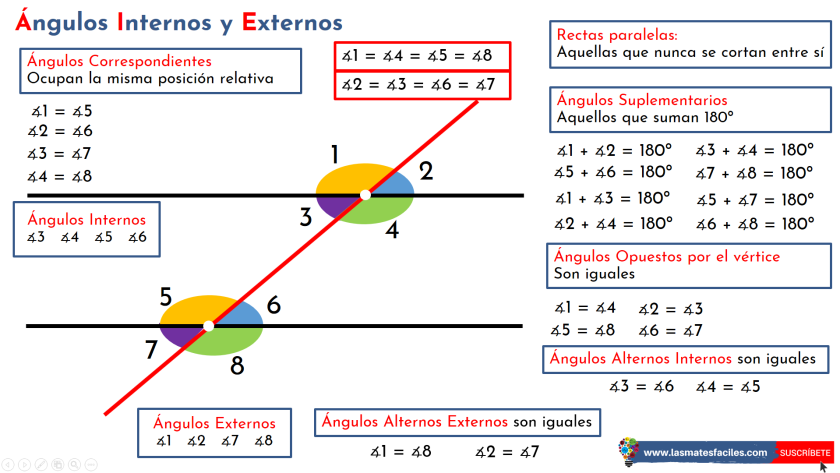
\includegraphics[width=17cm]{images/angulos 1}
    \caption{Teoremas sobre paralelismo.}
\end{figure}





\section{\large Unidad II. Calculo de área de Triángulos y Cuadriláteros}

\textbf{Definición:} Un \textbf{triángulo} es la unión de tres puntos (digamos $A, B, C$) no colineales.

\begin{enumerate}
    \item Dichos puntos se llaman \textbf{vértices} del triángulo.
    \item Los segmentos formados con dichos puntos, $AB, BC, AC$ se llaman \textbf{lados} del triángulo.
    \item Todo triángulo determina tres ángulos $\angle A, \angle B, \angle C$, llamados ángulos internos del triángulo.
    La suma de los ángulos siempre suman $180^\circ$, $\angle A + \angle B + \angle C = 180^\circ$.
    \item La suma de los lados de un triángulo se llama \textbf{perímetro} del triángulo.
\end{enumerate}


\textbf{Clasificación de triángulos}

\begin{enumerate}
    \item \textbf{Triángulo isósceles} es un triángulo con dos lados iguales y angulos correspondientes iguales ($a = c$ y $\angle A = \angle C$).
    \begin{figure}[htb]
        \centering
        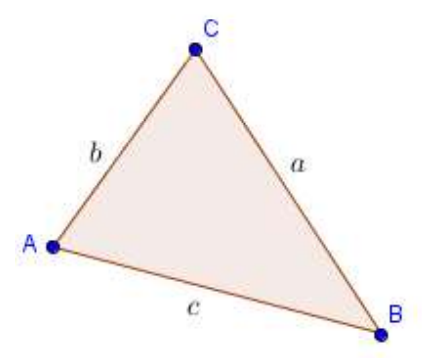
\includegraphics[width=4cm]{images/isosceles}
    \end{figure}
    \item \textbf{Triángulo equilátero} es un triángulo que tiene sus tres lados congurentes y sus tres angulos congruentes ($a = b = c$ y $\angle A = \angle B = \angle C$).
    \begin{figure}[htb]
        \centering
        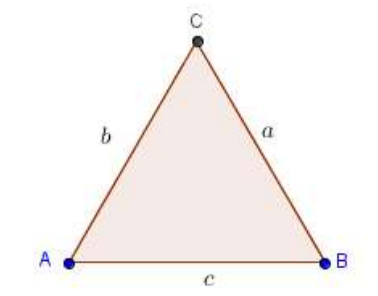
\includegraphics[width=4cm]{images/equilatero}
    \end{figure}
    \item \textbf{Triángulo rectángulo} es un triángulo que tiene un ángulo recto.
    El lado opuesto al ángulo recto se llama \textbf{hipotenusa} y al los otros dos lados se les llama \textbf{catetos}. ($AC$ es la hipotenusa y $AB, BC$ son los catetos)
    \begin{figure}[htb]
        \centering
        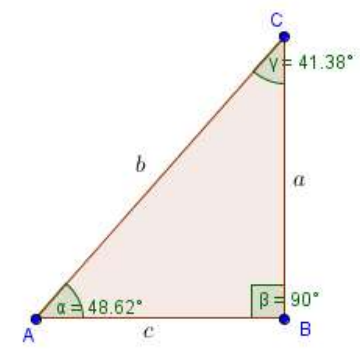
\includegraphics[width=5cm]{images/rectangulo}
    \end{figure}
    \item \textbf{Triángulo acutángulo} es un triángulo que tiene sus tres ángulos agudos y se \textbf{obtusángulo} si tiene un ángulo obtuso. (Ejemplo de acutangulo los primeros dos triángulos, ejemplode obtusangulo el siguinte triangulo)
    \begin{figure}[H]
        \centering
        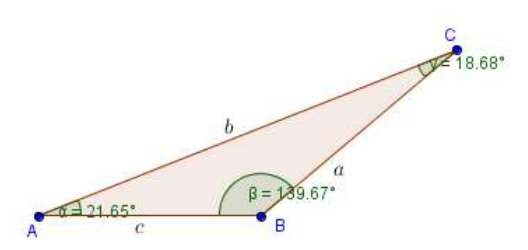
\includegraphics[width=5cm]{images/obtusangulo}
    \end{figure}
\end{enumerate}


\textbf{Congruencia de triángulos}

\begin{enumerate}
    \item \textbf{ALA (Ángulo - Lado - Ángulo)} Dos triángulos son congruentes si tiene congruentes un lado y los ángulos adyacentes a él.
     \begin{figure}[htb]
         \centering
         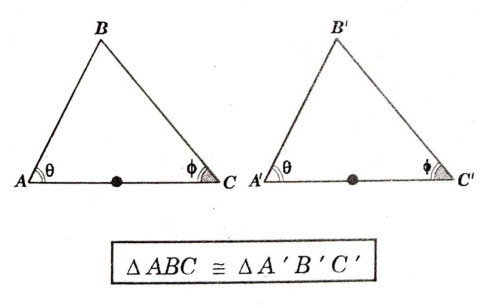
\includegraphics[width=7cm]{images/ala}
     \end{figure}
    \item \textbf{LAL (Lado - Ángulo - Lado)} Dos triángulos son congruentes si tienen congruentes dos lados y el ángulo comprendido entre ellos.
    \begin{figure}[htb]
        \centering
        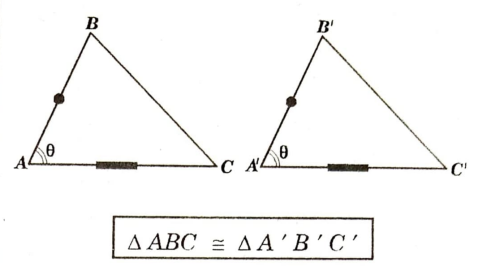
\includegraphics[width=7cm]{images/lal}
    \end{figure}
    \item \textbf{LLL (Lado - Lado - Lado)} Dos triángulos son congruentes si tienen congruentes sus tres lados congruentes respectivamente.
    \begin{figure}[htb]
        \centering
        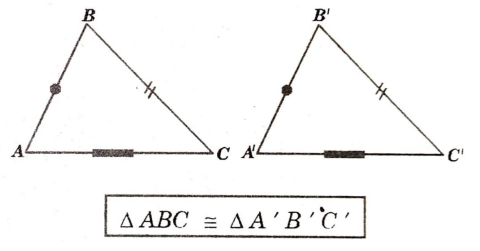
\includegraphics[width=7cm]{images/lll}
    \end{figure}
\end{enumerate}


\textbf{Cuadriláteros}

\textbf{Definición.} Un cuadrilátero es una figura cerrada de cuatro lados que se cortan unicamente en sus extremos.

\textbf{Clasificación de los cuadriláteros}
Una forma de clasificar los cuadriláteros es a partir del paralelismo de sus lados:
\begin{enumerate}
    \item \textbf{Paralelogramos:} son los cuadriláteros que tienen los dos pares de lados opuestos paralelos.
    \begin{figure}[H]
        \centering
        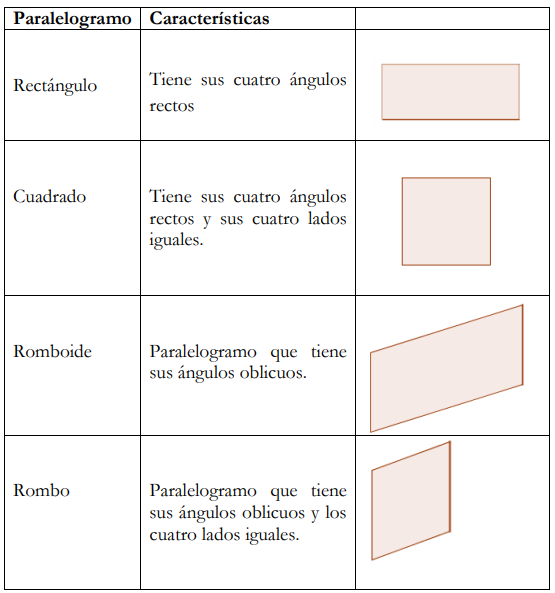
\includegraphics[width=12cm]{images/paralelogramo}
    \end{figure}
    \item \textbf{Trapecios:} son los cuadriláteros con una pareja de lados paralelos.
    \begin{figure}[H]
        \centering
        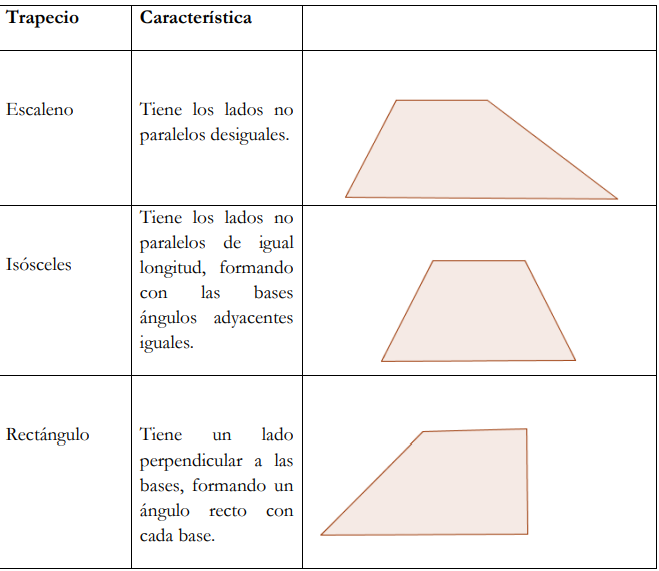
\includegraphics[width=12cm]{images/trapecio}
    \end{figure}
    \item \textbf{Trapezoides:} son los cuadriláteros que tienen no lados paralelos.
    \begin{figure}[H]
        \centering
        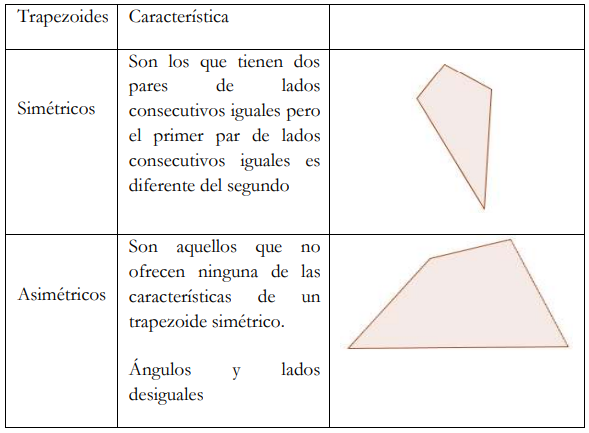
\includegraphics[width=12cm]{images/trapezoide}
    \end{figure}
\end{enumerate}



\textbf{Perimetros y áreas}

\begin{figure}[H]
    \centering
    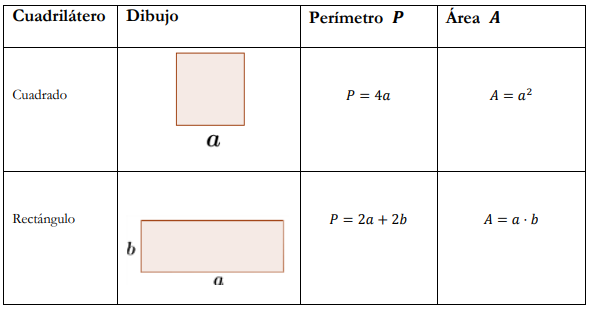
\includegraphics[width=12cm]{images/pya1}
\end{figure}

\begin{figure}[H]
    \centering
    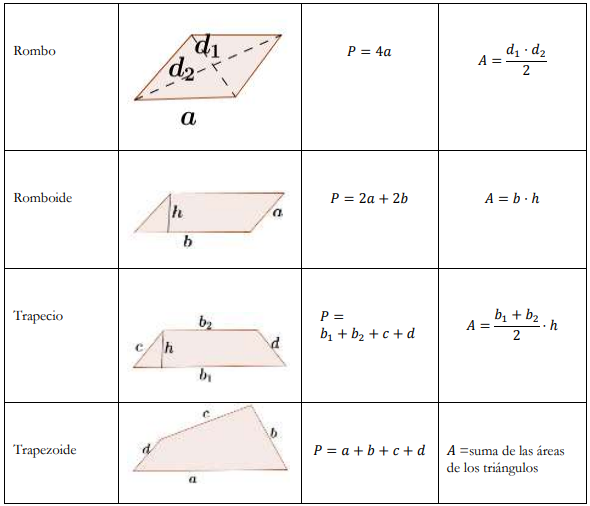
\includegraphics[width=12cm]{images/pya2}
\end{figure}




\section{\large Unidad III. Aplicaciones de la Geometría Analítica Vectorial}

\textbf{Definiciones:} Los vectores son magnitudes matematicas la cuales necesitan tres elementos para definirlas; magnitud, dirección y sentido.

Un vector se presentea graficamente mediante una flecha o segmento de dirigido.
Su magnitud se representa por el tamaño del segmento dirigido a una escala determinada y su dirección y sentido dado por la posición respecto a algún sistema de coordenada.

Simbolicamente puede representarse usando dos letras mayusculas (o bien una) con una flechita encima.

Ejemplo $\overrightarrow{AB}, \overrightarrow{PQ}$,etc, la primera letra representa el punto inicial y la segunda el punto terminal.

\textbf{Vectores iguales.} Dos vectores libres (aquellos que su punto inicial no está fijo) que tienen la misma magnitud y dirección se dice que son iguales sin que importe su posición en el espacio.

\begin{figure}[H]
    \centering
    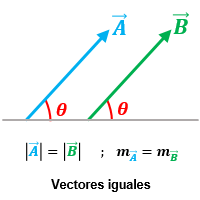
\includegraphics[width=6cm]{images/viguales}
\end{figure}

\textbf{El negativo u opuesto} de un vector $\overrightarrow{AB}$ es el vector que tiene igual magnitud que $\overrightarrow{AB}$, pero con sentido opuesto, se simboliza por $- \overrightarrow{AB}$ o $\overrightarrow{BA}$.

\textbf{Producto por un escalar o multiplo de un vector}

El producto del escalar $k$ por el vector $\overrightarrow{A}$, es el vector que tiene magnitud $k$ veces la de $\overrightarrow{A}$ y cuya dirección depende del signo algebraico de $k$.
\begin{figure}[H]
    \centering
    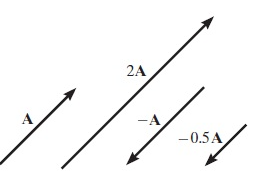
\includegraphics[width=6cm]{images/vproductoporescalar}
\end{figure}



\textbf{Suma de vectores}


\textbf{Método del triángulo}

La suma o resultante de dos vectores $\overrightarrow{A}$ y $\overrightarrow{B}$ es un vector $\overrightarrow{C}$ formado al colocar el punto inicial de $\overrightarrow{B}$ en el punto terminal de $\overrightarrow{A}$ y luego unir el punto inicial de $\overrightarrow{A}$ con el terminal de $\overrightarrow{B}$
\begin{figure}[H]
    \centering
    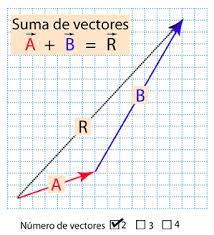
\includegraphics[width=6cm]{images/img}
\end{figure}


\textbf{Método del polígono}

Es una generalización del método del triángulo usado para sumar más de dos vectores.
En el punto final del primer vector, se traza el segundo vector; en el extremo de este se traza el tercer vector y así sucesivamente.
En cada caso la magnitud de cada vector está dada por la longitud de la flecha a una escala determinada.
La suma o resultante es el vector que va desde el punto inicial del primero al extremo final del último, es decir el que cierra el polígono, partiendo el punto inicial.

\begin{figure}[H]
    \centering
    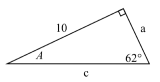
\includegraphics[width=6cm]{images/img_1}
\end{figure}